\section{Evaluation}
\subsection{Storage I/O test}

	Storage I/O is a key component for most scientific HPC applications. For example, large scale simulations need to first load large amount of data before processing and write back result after. Later, the result maybe used for other simulations. So I/O performance plays an important role for the overall performance of HPC application. In this section, we conduct experimental evaluation on storage I/O performance of BEE on HPC system. specially, we test and compare the performance of our three storage designs and native performance. To accurately evaluate storage I/O performance, we use benchmark tool IOR \cite{IOR}. We simulation the situation where there is one process per node and each process try to write and read 1GB of datafile stored in the shared storage directory using MPI-IO functions. To avoid inaccurate result cause by caching, each process only read files that is produced by other process on different node. 

\begin{figure}[h]
    \centering
    \caption{Storage I/O read test comparison on different storage designs of BEE}
    \label{io-test-read}
    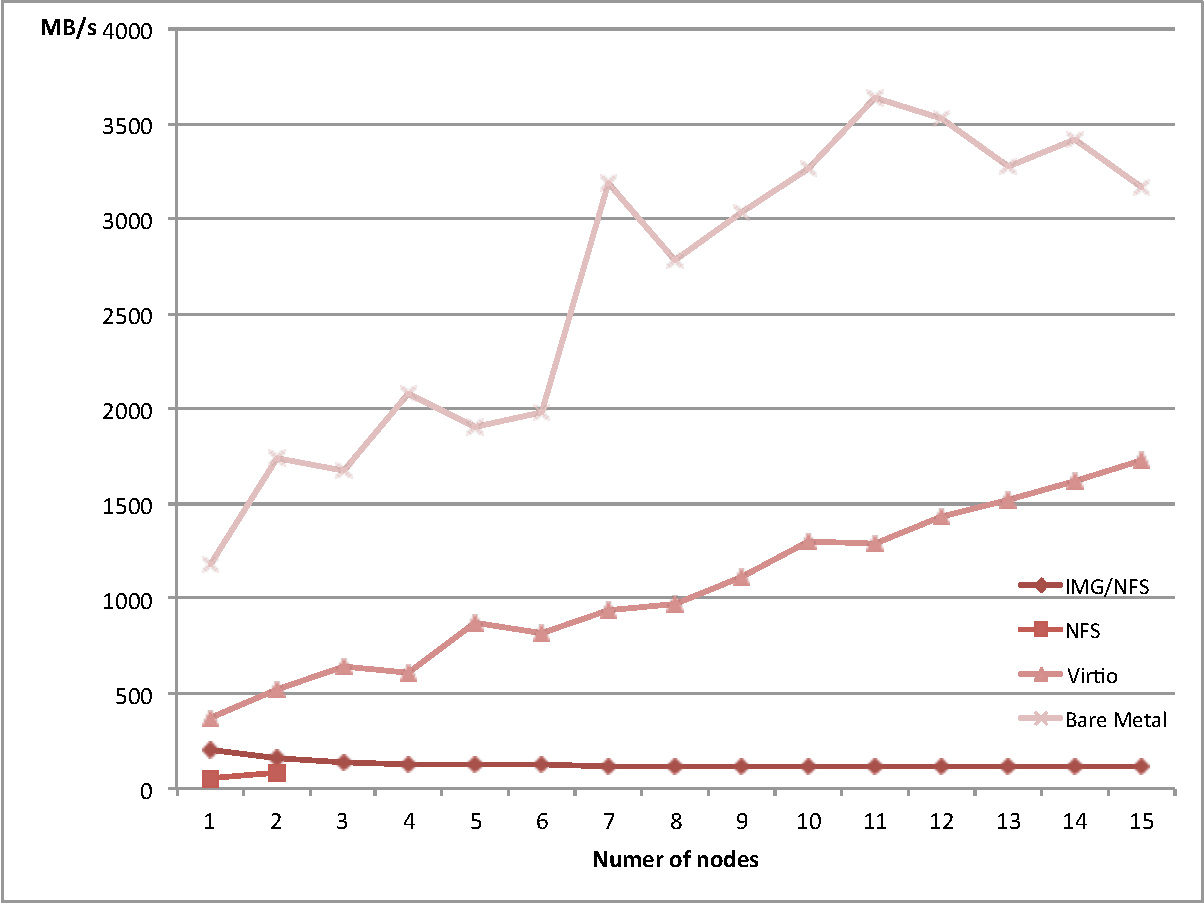
\includegraphics[width=0.5\textwidth]{figures/io-read-seq-test.pdf}
\end{figure}

\begin{figure}[h]
    \centering
    \caption{Storage I/O write test comparison on different storage designs of BEE}
    \label{io-test-write}
    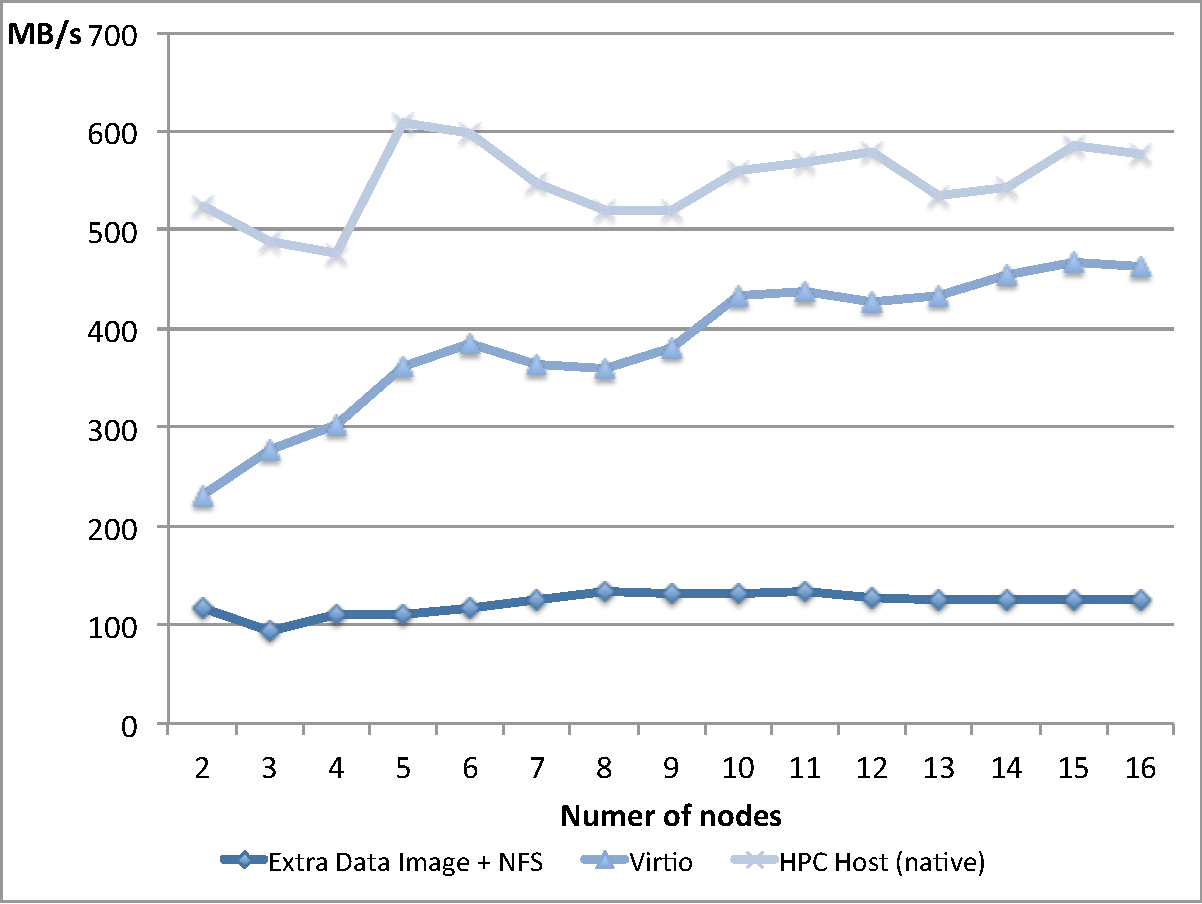
\includegraphics[width=0.5\textwidth]{figures/io-write-seq-test.pdf}
\end{figure}

The result is shown in \textbf{Figure \ref{io-test-read}} for read performance and \textbf{Figure \ref{io-test-write}} for write performance. \texttt{Data image + NFS} is the only node that does not rely on host file sharing abilities. When using \texttt{Data image + NFS} design, except the master node which directly mount the data image though hypervisor driver, other worker nodes all mount the shared directory through NFS, which depends on the network between master and worker. Since all I/O requests must go through the master node. The network performance of master node becomes the upper bound of storage I/O performance. As the number of worker nodes increases, master node becomes a hot spot which limits the overall I/O performance.  \texttt{NFS only} design offers the simplest setting. It doesn't require any special configuration except using mount command to mount host directory to local directory in virtual machines. It utilizes the first virtual NIC to connect to the host, so it does not occupy the network used for MPI communication. \texttt{Virtual IO} design utilizes the file system mapping feature of hypervisor. All storage I/O requests are sent to and processed by hypervisor driver. It offers the best performance and saves all network for MPI communication. As we can see in \textbf{Figure \ref{io-test-read}} and \textbf{\ref{io-test-write}}, this design can achieve almost half of the I/O read performance and 80\% I/O write performance of bare metal HPC system. They will continue to improve as we increase the number of nodes.

\subsection{Computing capability test}
Computing capability is another factor that need to be considered for running HPC applications. In this section, we compare the computing performance of HPC host with our virtualized BEE environment. To minimize other factors, we choose to run a compute intensive application, LU factorization, on a single multicore computing node with KVM enabled.

\begin{figure}[h]
    \centering
    \caption{Computing performance comparison between HPC host and BEE}
    \label{comp-test}
    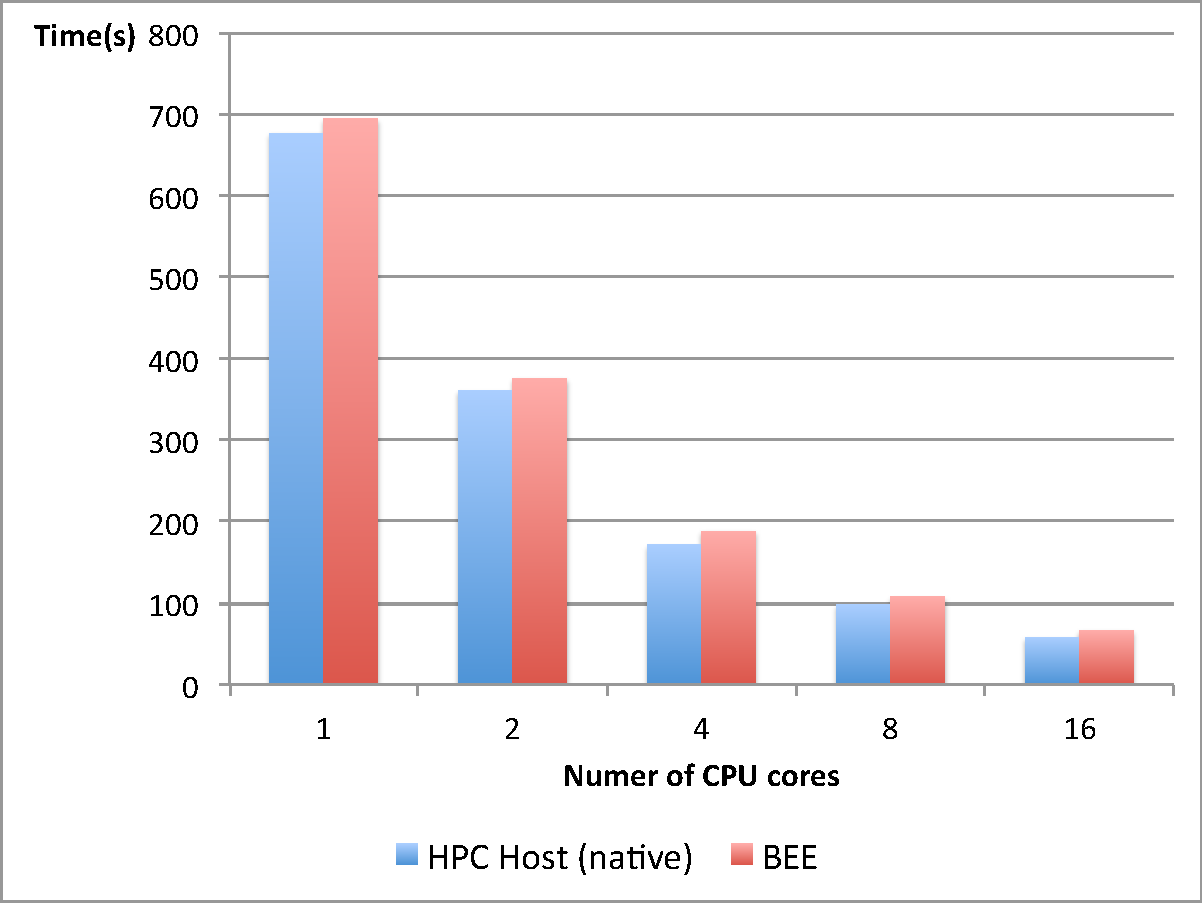
\includegraphics[width=0.5\textwidth]{figures/lu.pdf}
\end{figure}
 As shown in \textbf{Figure \ref{comp-test}}, although we brings two layers of virtuliazation for BEE, it only bring slightly overhead (approximately 9\%) to the HPC application. It also performs well in multicore environment. The overhead percentage almost stays constant as we increase the number of CPU cores.

